\chapter{Video Processing with GStreamer}
\label{chap:gstreamer}

\section{Motivation}
A significant amout of work was put into enabling on the fly compression of the videostreams from the \sr.
That is the ability to compress the video data as it is being recorded, and storing the compressed data on disk.

The sensor rig produces roughly 2Gib of data per second with a stereo camera setup.
At this rate, it will only take x days to produce a terabyte of data.
\begin{align}
    \frac{1\text{TB}}{2\text{Gb/s}} & = \frac{1\text{TB}}{0.25\text{GB/s}} \\
                                    & = 4000\text{s}                       \\
                                    & \approx 1\text{h} + 7\text{min}
\end{align}

It can be argued that datasets of this size is good enough, especially since it would also be possible to an \gls{ssd} with a capacity up to 8TB \cite{CorsairMP600PRO}, enabling roughly 9 hours of recording.
However, there are three reasons why on the fly compression is desirable:
If the sensor rig is mounted on a ship, it will be possible to transfer all the data to a storage server on the ship over regular ether net, using the ethernet port on the \jx which is limited to 1Gb/s.

By adjusting the compression rate of the sensor rig data can be transferred over ethernet for remote real time processing.
The compression has to be done at some point anyway.






% \begin{figure}
%     \centering
%     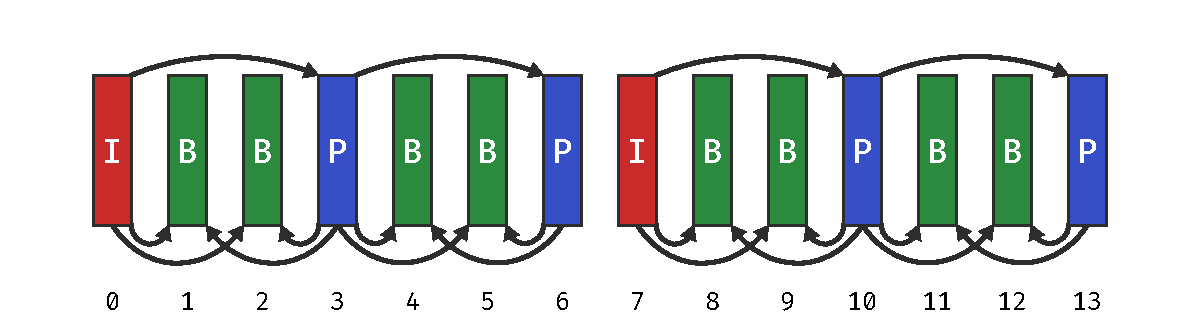
\includegraphics[width=0.8\textwidth]{figures/compression/ipb_frames.webp}
%     \caption{Frames}
%     \label{fig:ipbframes}
% \end{figure}